\documentclass[twoside]{book}

% Packages required by doxygen
\usepackage{fixltx2e}
\usepackage{calc}
\usepackage{doxygen}
\usepackage[export]{adjustbox} % also loads graphicx
\usepackage{graphicx}
\usepackage[utf8]{inputenc}
\usepackage{makeidx}
\usepackage{multicol}
\usepackage{multirow}
\PassOptionsToPackage{warn}{textcomp}
\usepackage{textcomp}
\usepackage[nointegrals]{wasysym}
\usepackage[table]{xcolor}

% Font selection
\usepackage[T1]{fontenc}
\usepackage[scaled=.90]{helvet}
\usepackage{courier}
\usepackage{amssymb}
\usepackage{sectsty}
\renewcommand{\familydefault}{\sfdefault}
\allsectionsfont{%
  \fontseries{bc}\selectfont%
  \color{darkgray}%
}
\renewcommand{\DoxyLabelFont}{%
  \fontseries{bc}\selectfont%
  \color{darkgray}%
}
\newcommand{\+}{\discretionary{\mbox{\scriptsize$\hookleftarrow$}}{}{}}

% Page & text layout
\usepackage{geometry}
\geometry{%
  a4paper,%
  top=2.5cm,%
  bottom=2.5cm,%
  left=2.5cm,%
  right=2.5cm%
}
\tolerance=750
\hfuzz=15pt
\hbadness=750
\setlength{\emergencystretch}{15pt}
\setlength{\parindent}{0cm}
\setlength{\parskip}{3ex plus 2ex minus 2ex}
\makeatletter
\renewcommand{\paragraph}{%
  \@startsection{paragraph}{4}{0ex}{-1.0ex}{1.0ex}{%
    \normalfont\normalsize\bfseries\SS@parafont%
  }%
}
\renewcommand{\subparagraph}{%
  \@startsection{subparagraph}{5}{0ex}{-1.0ex}{1.0ex}{%
    \normalfont\normalsize\bfseries\SS@subparafont%
  }%
}
\makeatother

% Headers & footers
\usepackage{fancyhdr}
\pagestyle{fancyplain}
\fancyhead[LE]{\fancyplain{}{\bfseries\thepage}}
\fancyhead[CE]{\fancyplain{}{}}
\fancyhead[RE]{\fancyplain{}{\bfseries\leftmark}}
\fancyhead[LO]{\fancyplain{}{\bfseries\rightmark}}
\fancyhead[CO]{\fancyplain{}{}}
\fancyhead[RO]{\fancyplain{}{\bfseries\thepage}}
\fancyfoot[LE]{\fancyplain{}{}}
\fancyfoot[CE]{\fancyplain{}{}}
\fancyfoot[RE]{\fancyplain{}{\bfseries\scriptsize Generated by Doxygen }}
\fancyfoot[LO]{\fancyplain{}{\bfseries\scriptsize Generated by Doxygen }}
\fancyfoot[CO]{\fancyplain{}{}}
\fancyfoot[RO]{\fancyplain{}{}}
\renewcommand{\footrulewidth}{0.4pt}
\renewcommand{\chaptermark}[1]{%
  \markboth{#1}{}%
}
\renewcommand{\sectionmark}[1]{%
  \markright{\thesection\ #1}%
}

% Indices & bibliography
\usepackage{natbib}
\usepackage[titles]{tocloft}
\setcounter{tocdepth}{3}
\setcounter{secnumdepth}{5}
\makeindex

% Hyperlinks (required, but should be loaded last)
\usepackage{ifpdf}
\ifpdf
  \usepackage[pdftex,pagebackref=true]{hyperref}
\else
  \usepackage[ps2pdf,pagebackref=true]{hyperref}
\fi
\hypersetup{%
  colorlinks=true,%
  linkcolor=blue,%
  citecolor=blue,%
  unicode%
}

% Custom commands
\newcommand{\clearemptydoublepage}{%
  \newpage{\pagestyle{empty}\cleardoublepage}%
}

\usepackage{caption}
\captionsetup{labelsep=space,justification=centering,font={bf},singlelinecheck=off,skip=4pt,position=top}

%===== C O N T E N T S =====

\begin{document}

% Titlepage & ToC
\hypersetup{pageanchor=false,
             bookmarksnumbered=true,
             pdfencoding=unicode
            }
\pagenumbering{alph}
\begin{titlepage}
\vspace*{7cm}
\begin{center}%
{\Large My Project }\\
\vspace*{1cm}
{\large Generated by Doxygen 1.8.14}\\
\end{center}
\end{titlepage}
\clearemptydoublepage
\pagenumbering{roman}
\tableofcontents
\clearemptydoublepage
\pagenumbering{arabic}
\hypersetup{pageanchor=true}

%--- Begin generated contents ---
\chapter{Wiki4\+Food}
\label{md_controllers_readme}
\Hypertarget{md_controllers_readme}
It \textquotesingle{}s quiet upset and had been trouble for many of people to figure out the ideas of food/cuisine that going to eat,especially for the traveler/exchange student like me and which restaurant should go for in our daily life.\+However, integrated with Zomato A\+PI ,Google Map A\+PI and Edamam A\+PI,this project aims for provided the ideas for those persion who didn \textquotesingle{}t have any idea for their lunch/dinner,in which proivded them some suggestions according to the online recipe offered from Edamam A\+PI , also suggested some restaurants regards for those dishes by Zomato A\+PI and through Google Map A\+PI to represents the exact location by latitude offered from Zomato A\+PI.

 Zomato A\+PI , Edamam Recipe A\+PI,  Google Map A\+PI

\subsection*{flow chart of the functions}



\subsection*{Technological Specification}

\subsubsection*{front end development tool}

Vue.\+js is used for the project \textquotesingle{}s frontend architecture.\+As well as its flexbility and also strong resource fulfillment and support,supported together with Vuetify Framework,which is a material based design framework

\subsubsection*{backend development}

P\+HP with laravel/\+Code\+Igniter would be used as its M\+VC Structure and its convience to corp with A\+PI struff with Curl/\+O\+Auth 2.\+0,and easier to managed json afterwards.

\subsubsection*{Testing}

In terms of testing,Selnimum would be used as it supports with multiple platforms,the work that we assume the covered rates should be high(Usually About 60-\/70\% for coverage in large scale web development for success commerical products).

\subsubsection*{Version Control}

Git would be used and gitlab would be the platform that I did the version control.

\subsubsection*{Integration}

I would going to jenkin for continous integrate the project and help for testing.

\subsection*{Author}

Li Sing Lun,Gordon 
\chapter{Hierarchical Index}
\section{Class Hierarchy}
This inheritance list is sorted roughly, but not completely, alphabetically\+:\begin{DoxyCompactList}
\item \contentsline{section}{A\+P\+Irequest}{\pageref{class_a_p_irequest}}{}
\item C\+I\+\_\+\+Controller\begin{DoxyCompactList}
\item \contentsline{section}{Welcome}{\pageref{class_welcome}}{}
\end{DoxyCompactList}
\item \contentsline{section}{Food}{\pageref{class_food}}{}
\item Test\+Case\begin{DoxyCompactList}
\item \contentsline{section}{T\+D\+D\+D27\+Testing}{\pageref{class_t_d_d_d27_testing}}{}
\begin{DoxyCompactList}
\item \contentsline{section}{vocab}{\pageref{classvocab}}{}
\end{DoxyCompactList}
\end{DoxyCompactList}
\end{DoxyCompactList}

\chapter{Data Structure Index}
\section{Data Structures}
Here are the data structures with brief descriptions\+:\begin{DoxyCompactList}
\item\contentsline{section}{\mbox{\hyperlink{class_a_p_irequest}{A\+P\+Irequest}} }{\pageref{class_a_p_irequest}}{}
\item\contentsline{section}{\mbox{\hyperlink{class_food}{Food}} }{\pageref{class_food}}{}
\item\contentsline{section}{\mbox{\hyperlink{class_t_d_d_d27_testing}{T\+D\+D\+D27\+Testing}} }{\pageref{class_t_d_d_d27_testing}}{}
\item\contentsline{section}{\mbox{\hyperlink{classvocab}{vocab}} }{\pageref{classvocab}}{}
\item\contentsline{section}{\mbox{\hyperlink{class_welcome}{Welcome}} }{\pageref{class_welcome}}{}
\end{DoxyCompactList}

\chapter{File Index}
\section{File List}
Here is a list of all files with brief descriptions\+:\begin{DoxyCompactList}
\item\contentsline{section}{controllers/\mbox{\hyperlink{_a_p_irequest_8php}{A\+P\+Irequest.\+php}} }{\pageref{_a_p_irequest_8php}}{}
\item\contentsline{section}{controllers/\mbox{\hyperlink{_food_8php}{Food.\+php}} }{\pageref{_food_8php}}{}
\item\contentsline{section}{controllers/\mbox{\hyperlink{test_8php}{test.\+php}} }{\pageref{test_8php}}{}
\item\contentsline{section}{controllers/\mbox{\hyperlink{vocab_8php}{vocab.\+php}} }{\pageref{vocab_8php}}{}
\item\contentsline{section}{controllers/\mbox{\hyperlink{_welcome_8php}{Welcome.\+php}} }{\pageref{_welcome_8php}}{}
\end{DoxyCompactList}

\chapter{Data Structure Documentation}
\hypertarget{class_a_p_irequest}{}\section{A\+P\+Irequest Class Reference}
\label{class_a_p_irequest}\index{A\+P\+Irequest@{A\+P\+Irequest}}
\subsection*{Public Member Functions}
\begin{DoxyCompactItemize}
\item 
\mbox{\hyperlink{class_a_p_irequest_a65f97cf2471736a6999cefebea218a03}{file\+\_\+get\+\_\+contents\+\_\+curl\+\_\+z}} (\$url)
\item 
\mbox{\hyperlink{class_a_p_irequest_aa3376c3f771a5cb3ad5356d22674a5ad}{file\+\_\+get\+\_\+contents\+\_\+curl\+\_\+eadam}} (\$url)
\end{DoxyCompactItemize}


\subsection{Member Function Documentation}
\mbox{\Hypertarget{class_a_p_irequest_aa3376c3f771a5cb3ad5356d22674a5ad}\label{class_a_p_irequest_aa3376c3f771a5cb3ad5356d22674a5ad}} 
\index{A\+P\+Irequest@{A\+P\+Irequest}!file\+\_\+get\+\_\+contents\+\_\+curl\+\_\+eadam@{file\+\_\+get\+\_\+contents\+\_\+curl\+\_\+eadam}}
\index{file\+\_\+get\+\_\+contents\+\_\+curl\+\_\+eadam@{file\+\_\+get\+\_\+contents\+\_\+curl\+\_\+eadam}!A\+P\+Irequest@{A\+P\+Irequest}}
\subsubsection{\texorpdfstring{file\+\_\+get\+\_\+contents\+\_\+curl\+\_\+eadam()}{file\_get\_contents\_curl\_eadam()}}
{\footnotesize\ttfamily file\+\_\+get\+\_\+contents\+\_\+curl\+\_\+eadam (\begin{DoxyParamCaption}\item[{}]{\$url }\end{DoxyParamCaption})}

Make c\+U\+RL request to the Edadam A\+PI Server and then return json format files.


\begin{DoxyParams}{Parameters}
{\em \$url} & -\/ the url for doing syncorization to A\+PI \\
\hline
{\em \$ch} & -\/ the curl seed for sending sync request \\
\hline
\end{DoxyParams}
\begin{DoxyReturn}{Returns}
json format data that sync from server
\end{DoxyReturn}
\mbox{\Hypertarget{class_a_p_irequest_a65f97cf2471736a6999cefebea218a03}\label{class_a_p_irequest_a65f97cf2471736a6999cefebea218a03}} 
\index{A\+P\+Irequest@{A\+P\+Irequest}!file\+\_\+get\+\_\+contents\+\_\+curl\+\_\+z@{file\+\_\+get\+\_\+contents\+\_\+curl\+\_\+z}}
\index{file\+\_\+get\+\_\+contents\+\_\+curl\+\_\+z@{file\+\_\+get\+\_\+contents\+\_\+curl\+\_\+z}!A\+P\+Irequest@{A\+P\+Irequest}}
\subsubsection{\texorpdfstring{file\+\_\+get\+\_\+contents\+\_\+curl\+\_\+z()}{file\_get\_contents\_curl\_z()}}
{\footnotesize\ttfamily file\+\_\+get\+\_\+contents\+\_\+curl\+\_\+z (\begin{DoxyParamCaption}\item[{}]{\$url }\end{DoxyParamCaption})}

Make c\+U\+RL request to the Zomato A\+PI Server and then return json format files. 
\begin{DoxyParams}{Parameters}
{\em \$header} & -\/ the user key definition \\
\hline
{\em \$header2} & -\/ the application type definition \\
\hline
\end{DoxyParams}
\begin{DoxyReturn}{Returns}
json format data sync from the server
\end{DoxyReturn}


The documentation for this class was generated from the following file\+:\begin{DoxyCompactItemize}
\item 
controllers/\mbox{\hyperlink{_a_p_irequest_8php}{A\+P\+Irequest.\+php}}\end{DoxyCompactItemize}

\hypertarget{class_food}{}\section{Food Class Reference}
\label{class_food}\index{Food@{Food}}
\subsection*{Public Member Functions}
\begin{DoxyCompactItemize}
\item 
\mbox{\hyperlink{class_food_a7a4815360caa28b9dd57e867b8c24134}{set\+Var}} (\$variable)
\item 
\mbox{\hyperlink{class_food_a369dc5ef69d748e8ff2c8164be651f93}{set\+Figure}} (\$fig)
\item 
\mbox{\hyperlink{class_food_a2af8add37797384585cae101fb8cbfe7}{get\+Image}} ()
\item 
\mbox{\hyperlink{class_food_a10f28e97c10ba7f766a5c88c2608795e}{set\+Image}} (\$Image)
\item 
\mbox{\hyperlink{class_food_ad05c558a85e707c2fabf068416a38be3}{get\+Rec}} ()
\item 
\mbox{\hyperlink{class_food_add8836563dee7d1e0a68cea374f2446f}{set\+Recipe}} (\$recipe2)
\item 
\mbox{\hyperlink{class_food_a6c5d100d3beccfae5646d3d481a156ed}{detail}} (\$variable)
\end{DoxyCompactItemize}


\subsection{Member Function Documentation}
\mbox{\Hypertarget{class_food_a6c5d100d3beccfae5646d3d481a156ed}\label{class_food_a6c5d100d3beccfae5646d3d481a156ed}} 
\index{Food@{Food}!detail@{detail}}
\index{detail@{detail}!Food@{Food}}
\subsubsection{\texorpdfstring{detail()}{detail()}}
{\footnotesize\ttfamily detail (\begin{DoxyParamCaption}\item[{}]{\$variable }\end{DoxyParamCaption})}

\mbox{\Hypertarget{class_food_a2af8add37797384585cae101fb8cbfe7}\label{class_food_a2af8add37797384585cae101fb8cbfe7}} 
\index{Food@{Food}!get\+Image@{get\+Image}}
\index{get\+Image@{get\+Image}!Food@{Food}}
\subsubsection{\texorpdfstring{get\+Image()}{getImage()}}
{\footnotesize\ttfamily get\+Image (\begin{DoxyParamCaption}{ }\end{DoxyParamCaption})}

\mbox{\Hypertarget{class_food_ad05c558a85e707c2fabf068416a38be3}\label{class_food_ad05c558a85e707c2fabf068416a38be3}} 
\index{Food@{Food}!get\+Rec@{get\+Rec}}
\index{get\+Rec@{get\+Rec}!Food@{Food}}
\subsubsection{\texorpdfstring{get\+Rec()}{getRec()}}
{\footnotesize\ttfamily get\+Rec (\begin{DoxyParamCaption}{ }\end{DoxyParamCaption})}

\mbox{\Hypertarget{class_food_a369dc5ef69d748e8ff2c8164be651f93}\label{class_food_a369dc5ef69d748e8ff2c8164be651f93}} 
\index{Food@{Food}!set\+Figure@{set\+Figure}}
\index{set\+Figure@{set\+Figure}!Food@{Food}}
\subsubsection{\texorpdfstring{set\+Figure()}{setFigure()}}
{\footnotesize\ttfamily set\+Figure (\begin{DoxyParamCaption}\item[{}]{\$fig }\end{DoxyParamCaption})}

\mbox{\Hypertarget{class_food_a10f28e97c10ba7f766a5c88c2608795e}\label{class_food_a10f28e97c10ba7f766a5c88c2608795e}} 
\index{Food@{Food}!set\+Image@{set\+Image}}
\index{set\+Image@{set\+Image}!Food@{Food}}
\subsubsection{\texorpdfstring{set\+Image()}{setImage()}}
{\footnotesize\ttfamily set\+Image (\begin{DoxyParamCaption}\item[{}]{\$\+Image }\end{DoxyParamCaption})}

\mbox{\Hypertarget{class_food_add8836563dee7d1e0a68cea374f2446f}\label{class_food_add8836563dee7d1e0a68cea374f2446f}} 
\index{Food@{Food}!set\+Recipe@{set\+Recipe}}
\index{set\+Recipe@{set\+Recipe}!Food@{Food}}
\subsubsection{\texorpdfstring{set\+Recipe()}{setRecipe()}}
{\footnotesize\ttfamily set\+Recipe (\begin{DoxyParamCaption}\item[{}]{\$recipe2 }\end{DoxyParamCaption})}

\mbox{\Hypertarget{class_food_a7a4815360caa28b9dd57e867b8c24134}\label{class_food_a7a4815360caa28b9dd57e867b8c24134}} 
\index{Food@{Food}!set\+Var@{set\+Var}}
\index{set\+Var@{set\+Var}!Food@{Food}}
\subsubsection{\texorpdfstring{set\+Var()}{setVar()}}
{\footnotesize\ttfamily set\+Var (\begin{DoxyParamCaption}\item[{}]{\$variable }\end{DoxyParamCaption})}



The documentation for this class was generated from the following file\+:\begin{DoxyCompactItemize}
\item 
controllers/\mbox{\hyperlink{_food_8php}{Food.\+php}}\end{DoxyCompactItemize}

\hypertarget{class_t_d_d_d27_testing}{}\section{T\+D\+D\+D27\+Testing Class Reference}
\label{class_t_d_d_d27_testing}\index{T\+D\+D\+D27\+Testing@{T\+D\+D\+D27\+Testing}}
Inheritance diagram for T\+D\+D\+D27\+Testing\+:\begin{figure}[H]
\begin{center}
\leavevmode
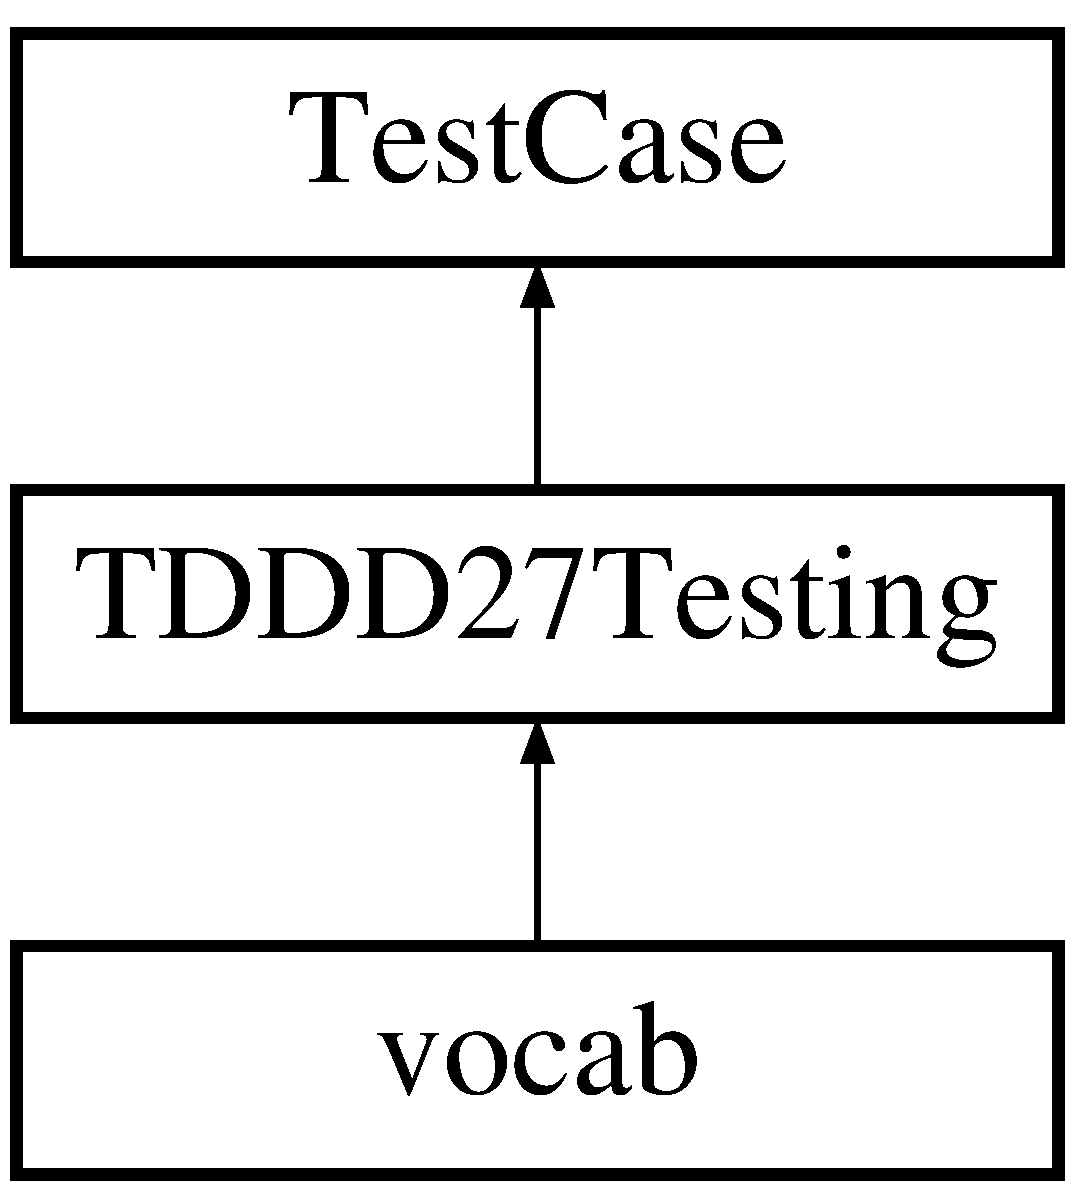
\includegraphics[height=3.000000cm]{class_t_d_d_d27_testing}
\end{center}
\end{figure}
\subsection*{Public Member Functions}
\begin{DoxyCompactItemize}
\item 
\mbox{\hyperlink{class_t_d_d_d27_testing_ae83d30c3504bfedb0c0d95ae76250b59}{test\+A\+P\+Ikeylocationidentification}} ()
\item 
\mbox{\hyperlink{class_t_d_d_d27_testing_ab0a2313acbb42c73e5b9f1f217f708a2}{test\+A\+P\+Ikeylocationinformation}} ()
\end{DoxyCompactItemize}


\subsection{Detailed Description}
Class used for perform Unit Testing

test if you run the following in the bash/\+Mac \+: ./phpunit --bootstrap ../../vendor/autoload.php test --debug 

\subsection{Member Function Documentation}
\mbox{\Hypertarget{class_t_d_d_d27_testing_ae83d30c3504bfedb0c0d95ae76250b59}\label{class_t_d_d_d27_testing_ae83d30c3504bfedb0c0d95ae76250b59}} 
\index{T\+D\+D\+D27\+Testing@{T\+D\+D\+D27\+Testing}!test\+A\+P\+Ikeylocationidentification@{test\+A\+P\+Ikeylocationidentification}}
\index{test\+A\+P\+Ikeylocationidentification@{test\+A\+P\+Ikeylocationidentification}!T\+D\+D\+D27\+Testing@{T\+D\+D\+D27\+Testing}}
\subsubsection{\texorpdfstring{test\+A\+P\+Ikeylocationidentification()}{testAPIkeylocationidentification()}}
{\footnotesize\ttfamily test\+A\+P\+Ikeylocationidentification (\begin{DoxyParamCaption}{ }\end{DoxyParamCaption})}

test\+A\+P\+Ikeylocation -\/ testing Zomato A\+PI location identication found whether works\mbox{\Hypertarget{class_t_d_d_d27_testing_ab0a2313acbb42c73e5b9f1f217f708a2}\label{class_t_d_d_d27_testing_ab0a2313acbb42c73e5b9f1f217f708a2}} 
\index{T\+D\+D\+D27\+Testing@{T\+D\+D\+D27\+Testing}!test\+A\+P\+Ikeylocationinformation@{test\+A\+P\+Ikeylocationinformation}}
\index{test\+A\+P\+Ikeylocationinformation@{test\+A\+P\+Ikeylocationinformation}!T\+D\+D\+D27\+Testing@{T\+D\+D\+D27\+Testing}}
\subsubsection{\texorpdfstring{test\+A\+P\+Ikeylocationinformation()}{testAPIkeylocationinformation()}}
{\footnotesize\ttfamily test\+A\+P\+Ikeylocationinformation (\begin{DoxyParamCaption}{ }\end{DoxyParamCaption})}

test\+A\+P\+Ikeylocationinformation -\/ testing Zomato A\+PI location and related information whether works

The documentation for this class was generated from the following file\+:\begin{DoxyCompactItemize}
\item 
controllers/\mbox{\hyperlink{test_8php}{test.\+php}}\end{DoxyCompactItemize}

\hypertarget{classvocab}{}\section{vocab Class Reference}
\label{classvocab}\index{vocab@{vocab}}
Inheritance diagram for vocab\+:\begin{figure}[H]
\begin{center}
\leavevmode
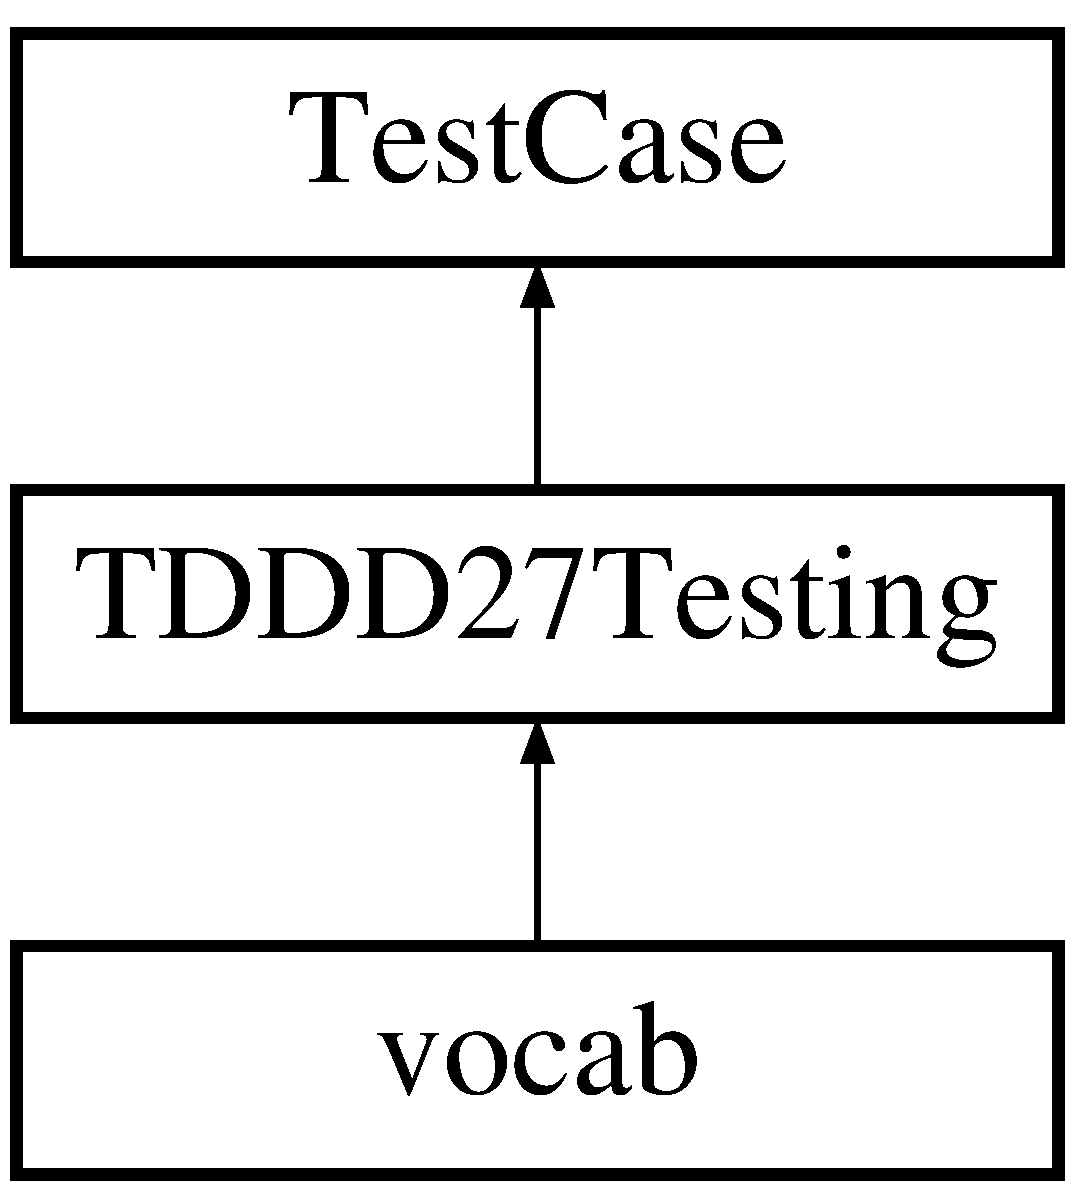
\includegraphics[height=3.000000cm]{classvocab}
\end{center}
\end{figure}
\subsection*{Public Member Functions}
\begin{DoxyCompactItemize}
\item 
\mbox{\hyperlink{classvocab_a154d9bd15e3326b9d91eaec11e4f4962}{keysydney}} ()
\item 
\mbox{\hyperlink{classvocab_a0ec3bfa6a46eb82117bc585e3f4ae367}{key\+London}} ()
\item 
\mbox{\hyperlink{classvocab_ac3a6124a50423e286b4c73dc2daf0aa4}{expectlondon}} ()
\item 
\mbox{\hyperlink{classvocab_a4741a8bc50fd4f346d8671e4cfd99bf7}{expectsydney}} ()
\end{DoxyCompactItemize}


\subsection{Member Function Documentation}
\mbox{\Hypertarget{classvocab_ac3a6124a50423e286b4c73dc2daf0aa4}\label{classvocab_ac3a6124a50423e286b4c73dc2daf0aa4}} 
\index{vocab@{vocab}!expectlondon@{expectlondon}}
\index{expectlondon@{expectlondon}!vocab@{vocab}}
\subsubsection{\texorpdfstring{expectlondon()}{expectlondon()}}
{\footnotesize\ttfamily expectlondon (\begin{DoxyParamCaption}{ }\end{DoxyParamCaption})}

\begin{DoxyReturn}{Returns}
expected output for London when load Zomato Location A\+PI 
\end{DoxyReturn}
\mbox{\Hypertarget{classvocab_a4741a8bc50fd4f346d8671e4cfd99bf7}\label{classvocab_a4741a8bc50fd4f346d8671e4cfd99bf7}} 
\index{vocab@{vocab}!expectsydney@{expectsydney}}
\index{expectsydney@{expectsydney}!vocab@{vocab}}
\subsubsection{\texorpdfstring{expectsydney()}{expectsydney()}}
{\footnotesize\ttfamily expectsydney (\begin{DoxyParamCaption}{ }\end{DoxyParamCaption})}

\begin{DoxyReturn}{Returns}
expected output for Sydney when load Zomato Location A\+PI 
\end{DoxyReturn}
\mbox{\Hypertarget{classvocab_a0ec3bfa6a46eb82117bc585e3f4ae367}\label{classvocab_a0ec3bfa6a46eb82117bc585e3f4ae367}} 
\index{vocab@{vocab}!key\+London@{key\+London}}
\index{key\+London@{key\+London}!vocab@{vocab}}
\subsubsection{\texorpdfstring{key\+London()}{keyLondon()}}
{\footnotesize\ttfamily key\+London (\begin{DoxyParamCaption}{ }\end{DoxyParamCaption})}

\begin{DoxyReturn}{Returns}
expected output for London when load location A\+PI 
\end{DoxyReturn}
\mbox{\Hypertarget{classvocab_a154d9bd15e3326b9d91eaec11e4f4962}\label{classvocab_a154d9bd15e3326b9d91eaec11e4f4962}} 
\index{vocab@{vocab}!keysydney@{keysydney}}
\index{keysydney@{keysydney}!vocab@{vocab}}
\subsubsection{\texorpdfstring{keysydney()}{keysydney()}}
{\footnotesize\ttfamily keysydney (\begin{DoxyParamCaption}{ }\end{DoxyParamCaption})}

\begin{DoxyReturn}{Returns}
expected output for sydney when load location A\+PI 
\end{DoxyReturn}


The documentation for this class was generated from the following file\+:\begin{DoxyCompactItemize}
\item 
controllers/\mbox{\hyperlink{vocab_8php}{vocab.\+php}}\end{DoxyCompactItemize}

\hypertarget{class_welcome}{}\section{Welcome Class Reference}
\label{class_welcome}\index{Welcome@{Welcome}}
Inheritance diagram for Welcome\+:\begin{figure}[H]
\begin{center}
\leavevmode
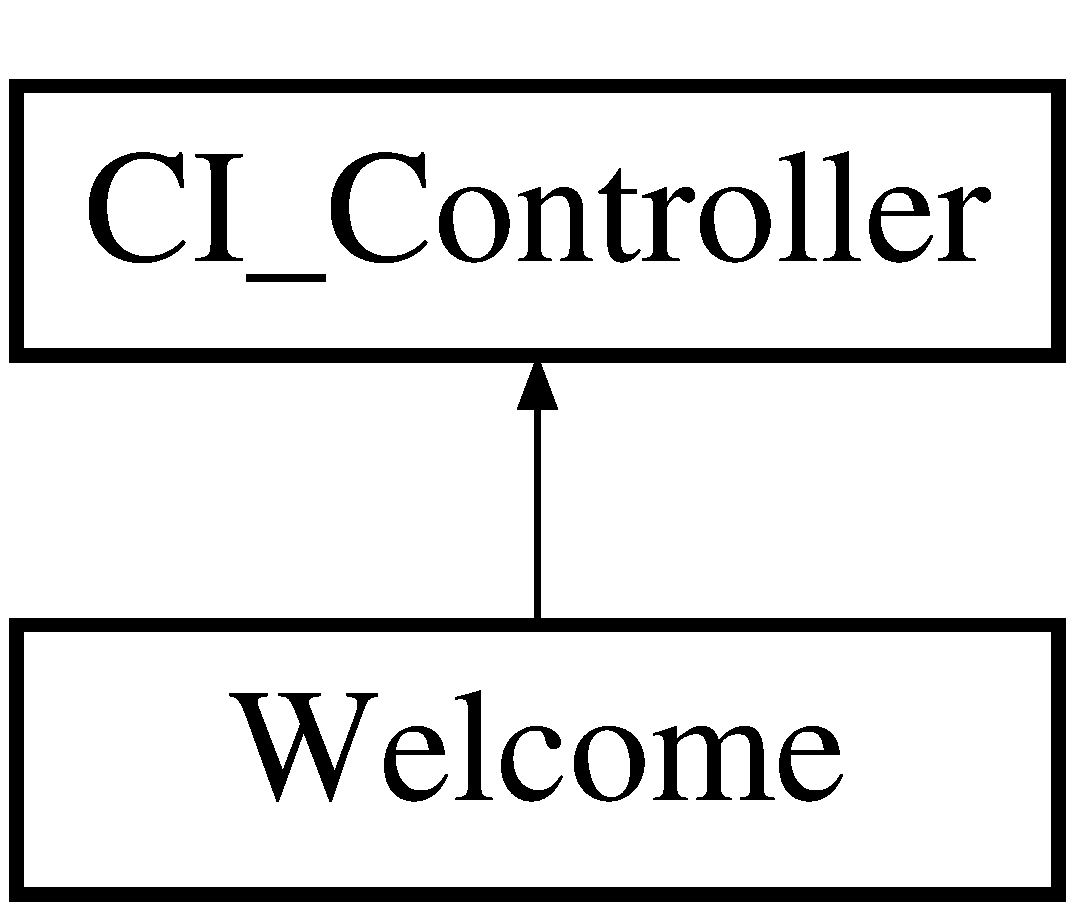
\includegraphics[height=2.000000cm]{class_welcome}
\end{center}
\end{figure}
\subsection*{Public Member Functions}
\begin{DoxyCompactItemize}
\item 
\mbox{\hyperlink{class_welcome_a149eb92716c1084a935e04a8d95f7347}{index}} ()
\item 
\mbox{\hyperlink{class_welcome_a76ab733fc756846ce6b6cdaddb8c005a}{adv\+Search}} ()
\item 
\mbox{\hyperlink{class_welcome_a4d5123cf815fd723d6dfdcb2c16fcc42}{form}} ()
\item 
\mbox{\hyperlink{class_welcome_a7edf443ddd63ae9348516d11b66d90a8}{sync\+Zomato\+Server}} (\$loc\+\_\+\+Read, \$cusine)
\item 
\mbox{\hyperlink{class_welcome_a1149321de0575cabb0e83f18de85728f}{location}} ()
\end{DoxyCompactItemize}


\subsection{Member Function Documentation}
\mbox{\Hypertarget{class_welcome_a76ab733fc756846ce6b6cdaddb8c005a}\label{class_welcome_a76ab733fc756846ce6b6cdaddb8c005a}} 
\index{Welcome@{Welcome}!adv\+Search@{adv\+Search}}
\index{adv\+Search@{adv\+Search}!Welcome@{Welcome}}
\subsubsection{\texorpdfstring{adv\+Search()}{advSearch()}}
{\footnotesize\ttfamily adv\+Search (\begin{DoxyParamCaption}{ }\end{DoxyParamCaption})}

advance search linkage

return to the adv\+Search\mbox{\Hypertarget{class_welcome_a4d5123cf815fd723d6dfdcb2c16fcc42}\label{class_welcome_a4d5123cf815fd723d6dfdcb2c16fcc42}} 
\index{Welcome@{Welcome}!form@{form}}
\index{form@{form}!Welcome@{Welcome}}
\subsubsection{\texorpdfstring{form()}{form()}}
{\footnotesize\ttfamily form (\begin{DoxyParamCaption}{ }\end{DoxyParamCaption})}

sync the request to Eadamam A\+PI and then used extract datum to represent in v-\/card format


\begin{DoxyParams}{Parameters}
{\em \$stmtheader} & -\/ header for api request \\
\hline
{\em \$stmtkey} & -\/ detail for default applicaiton request \\
\hline
{\em \$\+\_\+\+G\+E\+T\mbox{[}\char`\"{}search\char`\"{}\mbox{]}} & -\/ search data type come from the user \textquotesingle{}s default request \\
\hline
{\em \$oh} & -\/ object header of the the api request link \\
\hline
{\em \$linkedurl} & -\/ url link sent for request \\
\hline
{\em \$food} & -\/ object for storing the data ( try to use OO in programming) \\
\hline
{\em count} & -\/ the number of hits that users requested \\
\hline
{\em \$data\mbox{[}\textquotesingle{}image\textquotesingle{}\mbox{]}} & -\/ image of data \\
\hline
{\em \$data\mbox{[}\textquotesingle{}label\textquotesingle{}\mbox{]}} & -\/ label of dish \\
\hline
{\em \$data\mbox{[}\char`\"{}arr\char`\"{}\mbox{]}} & -\/ recipe of the disc\\
\hline
\end{DoxyParams}
\mbox{\Hypertarget{class_welcome_a149eb92716c1084a935e04a8d95f7347}\label{class_welcome_a149eb92716c1084a935e04a8d95f7347}} 
\index{Welcome@{Welcome}!index@{index}}
\index{index@{index}!Welcome@{Welcome}}
\subsubsection{\texorpdfstring{index()}{index()}}
{\footnotesize\ttfamily index (\begin{DoxyParamCaption}{ }\end{DoxyParamCaption})}

Index Page for this controller.

Maps to the following U\+RL \href{http://example.com/index.php/welcome}{\tt http\+://example.\+com/index.\+php/welcome}
\begin{DoxyItemize}
\item or -\/ \href{http://example.com/index.php/welcome/index}{\tt http\+://example.\+com/index.\+php/welcome/index}
\item or -\/ Since this controller is set as the default controller in config/routes.\+php, it\textquotesingle{}s displayed at \href{http://example.com/}{\tt http\+://example.\+com/}
\end{DoxyItemize}

So any other public methods not prefixed with an underscore will map to /index.php/welcome/$<$method\+\_\+name$>$ \begin{DoxySeeAlso}{See also}
\href{https://codeigniter.com/user_guide/general/urls.html}{\tt https\+://codeigniter.\+com/user\+\_\+guide/general/urls.\+html} 
\end{DoxySeeAlso}
index of the page

return the intorduction of the website\mbox{\Hypertarget{class_welcome_a1149321de0575cabb0e83f18de85728f}\label{class_welcome_a1149321de0575cabb0e83f18de85728f}} 
\index{Welcome@{Welcome}!location@{location}}
\index{location@{location}!Welcome@{Welcome}}
\subsubsection{\texorpdfstring{location()}{location()}}
{\footnotesize\ttfamily location (\begin{DoxyParamCaption}{ }\end{DoxyParamCaption})}

Grab the location by using Zomato A\+PI , datum of latitude and longtitude supported with Eadamai A\+PI. and using the Google M\+AP A\+PI to represent the datum into the map size. 
\begin{DoxyParams}{Parameters}
{\em \$address} & \\
\hline
{\em \$latitude} & \\
\hline
{\em \$longitude} & \\
\hline
{\em \$rating} & \\
\hline
{\em \$outlook} & \\
\hline
{\em \$placename} & \\
\hline
{\em \$data} & -\/ send buffer from controller to view\\
\hline
\end{DoxyParams}
\mbox{\Hypertarget{class_welcome_a7edf443ddd63ae9348516d11b66d90a8}\label{class_welcome_a7edf443ddd63ae9348516d11b66d90a8}} 
\index{Welcome@{Welcome}!sync\+Zomato\+Server@{sync\+Zomato\+Server}}
\index{sync\+Zomato\+Server@{sync\+Zomato\+Server}!Welcome@{Welcome}}
\subsubsection{\texorpdfstring{sync\+Zomato\+Server()}{syncZomatoServer()}}
{\footnotesize\ttfamily sync\+Zomato\+Server (\begin{DoxyParamCaption}\item[{}]{\$loc\+\_\+\+Read,  }\item[{}]{\$cusine }\end{DoxyParamCaption})}

Plug location and cusine type for specific your search, and then make a request to the Zomato server, finally return json key.


\begin{DoxyParams}{Parameters}
{\em headoflocation} & -\/ header of the zomato link \\
\hline
{\em src\+\_\+location} & -\/ linked to the method that get\+\_\+content \\
\hline
{\em buffer\+\_\+location} & -\/ buffer for storing the json styled file \\
\hline
{\em tail} & -\/ entity type definiton \\
\hline
{\em counting} & -\/ the number of data that want to show \\
\hline
{\em api} & -\/ the final api link want to going to sync \\
\hline
\end{DoxyParams}
\begin{DoxyReturn}{Returns}
-\/ json file type datum back to server and manage
\end{DoxyReturn}


The documentation for this class was generated from the following file\+:\begin{DoxyCompactItemize}
\item 
controllers/\mbox{\hyperlink{_welcome_8php}{Welcome.\+php}}\end{DoxyCompactItemize}

\chapter{File Documentation}
\hypertarget{_a_p_irequest_8php}{}\section{controllers/\+A\+P\+Irequest.php File Reference}
\label{_a_p_irequest_8php}\index{controllers/\+A\+P\+Irequest.\+php@{controllers/\+A\+P\+Irequest.\+php}}
\subsection*{Data Structures}
\begin{DoxyCompactItemize}
\item 
class \mbox{\hyperlink{class_a_p_irequest}{A\+P\+Irequest}}
\end{DoxyCompactItemize}

\hypertarget{_food_8php}{}\section{controllers/\+Food.php File Reference}
\label{_food_8php}\index{controllers/\+Food.\+php@{controllers/\+Food.\+php}}
\subsection*{Data Structures}
\begin{DoxyCompactItemize}
\item 
class \mbox{\hyperlink{class_food}{Food}}
\end{DoxyCompactItemize}

\hypertarget{readme_8md}{}\section{controllers/readme.md File Reference}
\label{readme_8md}\index{controllers/readme.\+md@{controllers/readme.\+md}}

\hypertarget{test_8php}{}\section{controllers/test.php File Reference}
\label{test_8php}\index{controllers/test.\+php@{controllers/test.\+php}}
\subsection*{Data Structures}
\begin{DoxyCompactItemize}
\item 
class \mbox{\hyperlink{class_t_d_d_d27_testing}{T\+D\+D\+D27\+Testing}}
\end{DoxyCompactItemize}

\hypertarget{vocab_8php}{}\section{controllers/vocab.php File Reference}
\label{vocab_8php}\index{controllers/vocab.\+php@{controllers/vocab.\+php}}
\subsection*{Data Structures}
\begin{DoxyCompactItemize}
\item 
class \mbox{\hyperlink{classvocab}{vocab}}
\end{DoxyCompactItemize}

\hypertarget{_welcome_8php}{}\section{controllers/\+Welcome.php File Reference}
\label{_welcome_8php}\index{controllers/\+Welcome.\+php@{controllers/\+Welcome.\+php}}
\subsection*{Data Structures}
\begin{DoxyCompactItemize}
\item 
class \mbox{\hyperlink{class_welcome}{Welcome}}
\end{DoxyCompactItemize}

%--- End generated contents ---

% Index
\backmatter
\newpage
\phantomsection
\clearemptydoublepage
\addcontentsline{toc}{chapter}{Index}
\printindex

\end{document}
